\section{Auswertung}
\subsection{Vorgehen und genutzte Programme}
Zur Automatisierung der Auswertung wird wie folgt vorgegangen:
\begin{enumerate}
  \item Die Filme werden auf einem Scanner digitalisiert.
  Der Film der Salzprobe muss dabei während des scannens von oben beleuchtet werden,
  da der Film durch die längere Messdauer und Streulicht sehr stark belichtet
  wurde.
  \item Die gescannten Bilder werden digital nachbearbeitet, sodass die
  Beugungskreise besser hervortreten.
  \item Zwischen den Stanzungen der Filme werden die Grauwerte in einem schmalen,
  mittigen Streifen ausgelesen.
  Dazu wird das Programm ImageJ\cite{Schneider2012} genutzt.
  \item Die Grauwerte werden in einem Python\cite{python}-script
  durch Pandas\cite{mckinney-proc-scipy-2010} eingelesen.
  Der Grauwert wird invertiert und der Untergrund manuell auf ein
  einheitliches Niveau zu heben.
  \item Durch die Funktion \texttt{find\_peaks} der SciPy\cite{scipy}-Bibliothek
  \texttt{signal} werden die Peaks und damit die Beugungskreise detektiert.
  Die Abstände zum Mittelpunkt der Stanzung in Millimeter entsprechen dabei
  dem Winkel in Grad.
  \item Für jeden Peak werden durch die Bragggleichung Netzebenenabstände
  berechnet. Durch Vergleich mit jedem möglichen Tupel von Millerindizes
  (bis zu einem Wert $\text{max}(h, \, k, \, l) = 7$) wird der bestmögliche
  Wert für die Gitterkonstante bestimmt, indem die Abweichungen der Gitterkonstanten
  untereinander minimiert werden. Dies wird für ein fcc- und ein bcc-Gitter getan.
  \item Durch die SciPy-optimize Funktion \texttt{curve\_fit} wird ein linearer
  Fit durch die Gitterkonstanten beider Gittertypen gelegt und der optimale Wert
  durch den y-Achsenabschnitt bestimmt.
\end{enumerate}

\subsection{Metallprobe}
Der Ausschnitt zwischen den Stanzungen des Films ist in \autoref{Abb:Metall}
zu sehen, die ausgelesenen Reflexe finden sich in \autoref{Tab:Metall}.

\begin{figure}
  \centering
  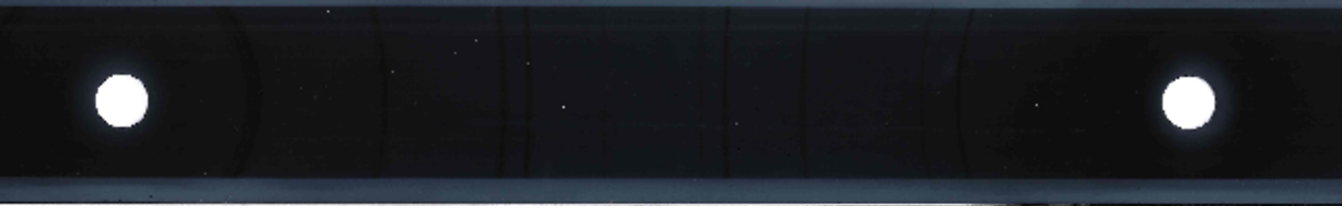
\includegraphics[scale=0.5]{content/pics/Metall_film.pdf}
  \caption{Filmaufnahme der Metallprobe.}
  \label{Abb:Metall}
\end{figure}

\begin{table}[H]
  \centering
  \caption{Beugungsreflexe an der Metallprobe und zugeordnete Millerindizes für bcc und fcc-Gitter.}
  \label{Tab:Metall}
  \begin{tabular}{c || c c | c c}
    \toprule
    Winkel / ° & $(h, \, k, \, l)_{\text{bcc}}$ & $a_{\text{bcc}}$ / pm & $(h, \, k, \, l)_{\text{fcc}}$ & $a_{\text{fcc}}$\\
    \midrule
    40.35 & 2 & 1 & 1 & 0 & 315.92 & 3 & 1 & 1 & 1 & 386.92 \\
46.32 & 4 & 2 & 0 & 0 & 391.83 & 4 & 2 & 0 & 0 & 391.83 \\
65.61 & 6 & 2 & 1 & 1 & 348.32 & 8 & 2 & 2 & 0 & 402.21 \\
79.65 & 8 & 2 & 2 & 0 & 340.27 & 11 & 3 & 1 & 1 & 399.00 \\
112.63 & 10 & 3 & 1 & 0 & 292.80 & 12 & 2 & 2 & 2 & 320.75 \\
116.84 & 12 & 2 & 2 & 2 & 313.29 & 16 & 4 & 0 & 0 & 361.75 \\
136.84 & 14 & 3 & 2 & 1 & 310.01 & 19 & 3 & 3 & 1 & 361.15 \\
158.60 & 16 & 4 & 0 & 0 & 313.64 & 20 & 4 & 2 & 0 & 350.66 \\

    \bottomrule
  \end{tabular}
\end{table}

\subsection{Salzprobe}

\begin{figure}
  \centering
  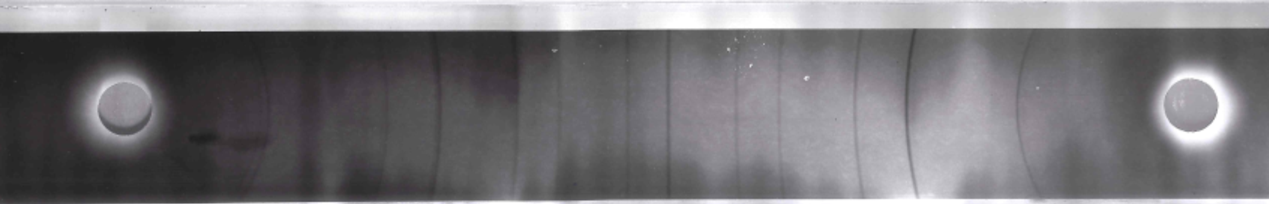
\includegraphics[scale=0.5]{content/pics/Salz_film.pdf}
  \caption{Filmaufnahme der Metallprobe.}
  \label{Abb:Salz}
\end{figure}

\begin{table}[H]
  \centering
  \caption{Beugungsreflexe and der Salzprobe und zugeordnete Millerindizes für bcc und fcc-Gitter.}
  \label{Tab:Salz}
  \begin{tabular}{c || c c | c c}
    \toprule
    Winkel / ° & $(h, \, k, \, l)_{\text{bcc}}$ & $a_{\text{bcc}}$ / pm & $(h, \, k, \, l)_{\text{fcc}}$ & $a_{\text{fcc}}$\\
    \midrule
    40.35 & 2 & 1 & 1 & 0 & 315.92 & 3 & 1 & 1 & 1 & 386.92 \\
46.32 & 4 & 2 & 0 & 0 & 391.83 & 4 & 2 & 0 & 0 & 391.83 \\
65.61 & 6 & 2 & 1 & 1 & 348.32 & 8 & 2 & 2 & 0 & 402.21 \\
79.65 & 8 & 2 & 2 & 0 & 340.27 & 11 & 3 & 1 & 1 & 399.00 \\
112.63 & 10 & 3 & 1 & 0 & 292.80 & 12 & 2 & 2 & 2 & 320.75 \\
116.84 & 12 & 2 & 2 & 2 & 313.29 & 16 & 4 & 0 & 0 & 361.75 \\
136.84 & 14 & 3 & 2 & 1 & 310.01 & 19 & 3 & 3 & 1 & 361.15 \\
158.60 & 16 & 4 & 0 & 0 & 313.64 & 20 & 4 & 2 & 0 & 350.66 \\

    \bottomrule
  \end{tabular}
\end{table}

\section{Diskusion}
